% Inbuilt themes in beamer
\documentclass{beamer}


%Defining some colours
\definecolor{darkred}{rgb}{0.8,0,0}

% Theme choice: there a number of preset themes to choose from
% Play around with them, Cambridge is nice for first pres
%\usetheme{Szeged}
\usetheme{CambridgeUS} %setting the main theme
\usecolortheme{whale} % setting colour theme
\usefonttheme{professionalfonts} %font theme
\useinnertheme[shadow=true]{rounded}
%\useoutertheme{} %outer theme

%\setbeamertemplate{footline} %Remove footer line in all slides
\setbeamertemplate{navigation symbols}{} %removes navigation symbols
\setbeamertemplate{footline}[page number] %removes footer line, keeps pg#
\setbeamertemplate{caption}{\insertcaption} 


%Setting colours for boxes and captions
\setbeamercolor{block title}{bg=blue!30, fg=black}
\setbeamercolor{block body}{bg=blue!10}
\setbeamercolor{frametitle}{fg=black}

%%%FOR VIDEOS
\usepackage{media9}
\usepackage{multimedia}
% For the Flowchart
%\usepackage{tikz}
%\usetikzlibrary{shapes.geometric, arrows}
%\tikzstyle{startstop} = [rectangle, rounded corners, minimum width=3cm, minimum height=1cm,text centered, draw=black, fill=blue!30]
%\tikzstyle{process} = [rectangle, minimum width=3cm, minimum height=1cm, text centered, draw=black, fill=orange!30]
%\tikzstyle{decision} = [diamond, minimum width=3cm, minimum height=1cm, text centered, draw=black, fill=green!30]
%\tikzstyle{arrow} = [thick,->,>=stealth]

%%% For the Timeline
\usepackage{xcolor}
\usepackage{tikz} \usetikzlibrary{calc, arrows.meta, intersections, patterns, positioning, shapes.misc, fadings, through,decorations.pathreplacing}

\definecolor{ColorOne}{rgb}{0.0,0.5,1.0} %Lightblue
\definecolor{ColorTwo}{rgb}{1.0,0.6,0.4} %lightorange
\definecolor{ColorThree}{rgb}{0.75,0.58,0.89} %lightpurple

% Title page details: 
\title[BEAP Dec 2022]{Current Affairs: Utilizing Oxford Nanopore Sequencing Data to Detect Non-Canonical DNA Structures} 
\author{Alexander Turco}
\date{\today}
\logo{
\includegraphics[height=0.5cm, width=3cm]{logo.png}}

% Bibliography stuff
\usepackage[natbib=true, sorting=nyt, style=authoryear-comp]{biblatex}
\addbibresource{ABC1.bib}

%Extra packages
\usepackage{makecell}

%For itemize
\setbeamertemplate{itemize item}[triangle]

%For Flow Chart
\usepackage{tikz}
\usetikzlibrary{shapes.geometric, arrows}

\tikzstyle{startstop} = [rectangle, 
minimum width=6cm, 
minimum height=1cm,
text centered, 
draw=black, 
fill=blue!30]

\tikzstyle{io} = [trapezium, 
trapezium stretches=true, % A later addition
trapezium left angle=70, 
trapezium right angle=110, 
minimum width=3cm, 
minimum height=1cm, text centered, 
draw=black, fill=blue!30]

\tikzstyle{process} = [rectangle, 
minimum width=3cm, 
minimum height=1cm, 
text align, 
text width=1cm, 
draw=black, 
fill=orange!30]

\tikzstyle{decision} = [diamond, 
minimum width=3cm, 
minimum height=1cm, 
text centered, 
draw=black, 
fill=green!30]
\tikzstyle{arrow} = [thick,->,>=stealth]

\begin{document}
	
	% For my introduction slides, there will be the slide with my title and name as well as an outline slide with the brief overview of what I will discuss.
	% Title page frame - SLIDE 1%%%%%%%%%%%%%%%%%%%%%%%%%%%%%%%%%%%%%%%%%%%%%%%%%%%%%%%%%%%%%%%%%%%%%%%%%%%%%%%%%%%%%%%%%%%%%%%%%%%%%%%%%%%%%%%%%%%%%%%%%%%%%%%%%%%%
	\section{Introduction}
	\begin{frame}
		\titlepage 
		\begin{center}
			%\includegraphics[width=7cm, height=4cm]{cellsatwar.png}
		\end{center}
	\end{frame}
	
	% Remove logo from the next slides
	\logo{}
	
	% Outline frame - SLIDE 2
	%\begin{frame}{Overview}
		
		%\begin{center}
		%\begin{minipage}{6cm}
				
		 % 		\begin{block}{} \hyperlink{link1}{Background Information} \end{block}
		  %		\begin{block}{} The Game Design Process \end{block}
		  %		\begin{block}{} Collection of Student Feedback \end{block}
		  %		\begin{block}{} Results \end{block}
		  		%\begin{block}{} Conclusions \end{block}
		  %		\begin{block}{} Future Work \end{block}

		%\end{minipage}
		%\end{center}
	
	%\end{frame}
	
	% For my Background slides, I will talk about important things such as WHat LCRs are, their evolution, stuff like that
	% SLIDE 3 - WHAT ARE LCRs%%%%%%%%%%%%%%%%%%%%%%%%%%%%%%%%%%%%%%%%%%%%%%%%%%%%%%%%%%%%%%%%%%%%%%%%%%%%%%%%%%%%%%%%%%%%%%%%%%%%%%%%%%%%%%%%%%%%%%%%%%%%%%%%%%%%%%
	% The graphic for this slide is an image of some output from segA with the parameters in the brackets
	\section{Background}
	\begin{frame}{The Structure of DNA: A Brief History Lesson}
		\begin{itemize}
			\item In 1953, Watson, Crick, Wilkins, Franklin, and Gosling were the first to describe the structure of DNA \newline
			\item They discovered the \textcolor{blue}{right-handed double helix} (canonical B-form DNA), the most common form found in cells \newline
		\end{itemize}
		
		\centering
		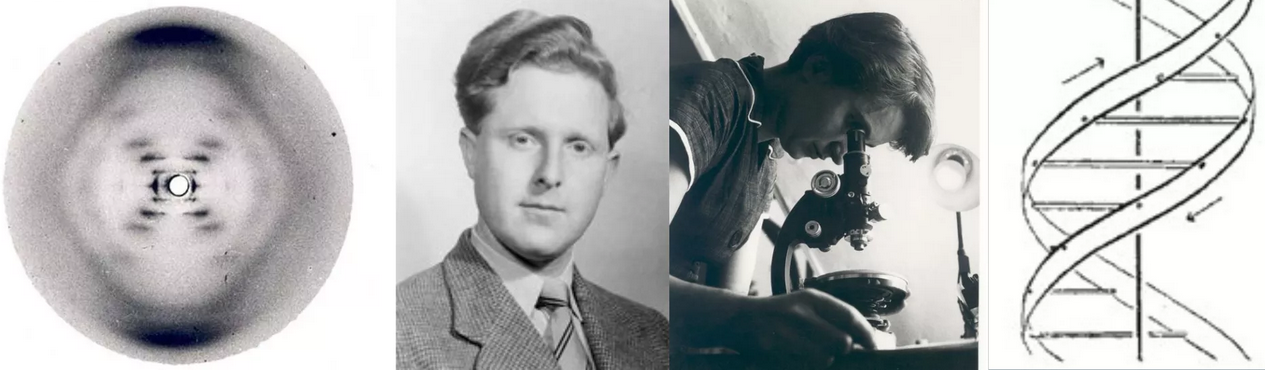
\includegraphics[width=11cm, height=3.5cm]{rosy.png}
		
		\footnotetext[1]{\tiny\cite{nijman2011synthetic}}
		
	\end{frame}
	
	%Also called synthetic sick because it can lead to reduced cell viability as opposed to death
	\begin{frame}{DNA Can Adopt Alternative Structures}
		\label{link1}
		
		\begin{itemize}
			\item Now, more than 15 types of DNA structure that differ from the canonical B-form have been reported (non-canonical or non-B form DNA) \newline
			\item Through sequencing of the human genome, we now know over half the genome is composed of repetitive elements - these were initially thought to be `junk DNA' \newline
			
			\begin{center}
				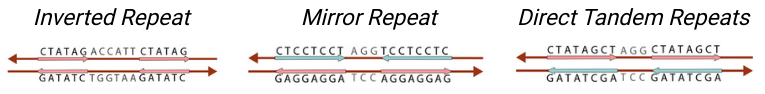
\includegraphics[width=9cm, height=1.2cm]{repeats.png}
			\end{center}
			 
			\item A crucial feature of some repetitive sequences is their ability to fold into non-canonical DNA structures (non-B DNA)
			\footnotetext[2]{\tiny\cite{lee2018harnessing}}
		\end{itemize}
		
	\end{frame}

	% SLIDE 4 - I do Not Know if I am including this slide
	% The Graphic for this slide is an  
	% Entropy, which is measured by Shannon's Entropy equation is a measure of compositional complexity which uses the proportion of residue(s)
	% in a subsequence to measure the compositional state of that subseequence - A lower variety of residues = lower entropy 
	%\begin{frame}{Shannon's Entropy - MAYBE }
		
	%		$H = -L\sum p_i log_2(p_i)$
		
	%\end{frame}

	%SLIDE 5 - LCR's PRESENT IN UNIQUE WAYS
	\begin{frame}{Types of Non-canonical DNA structures}
		
		\centering
		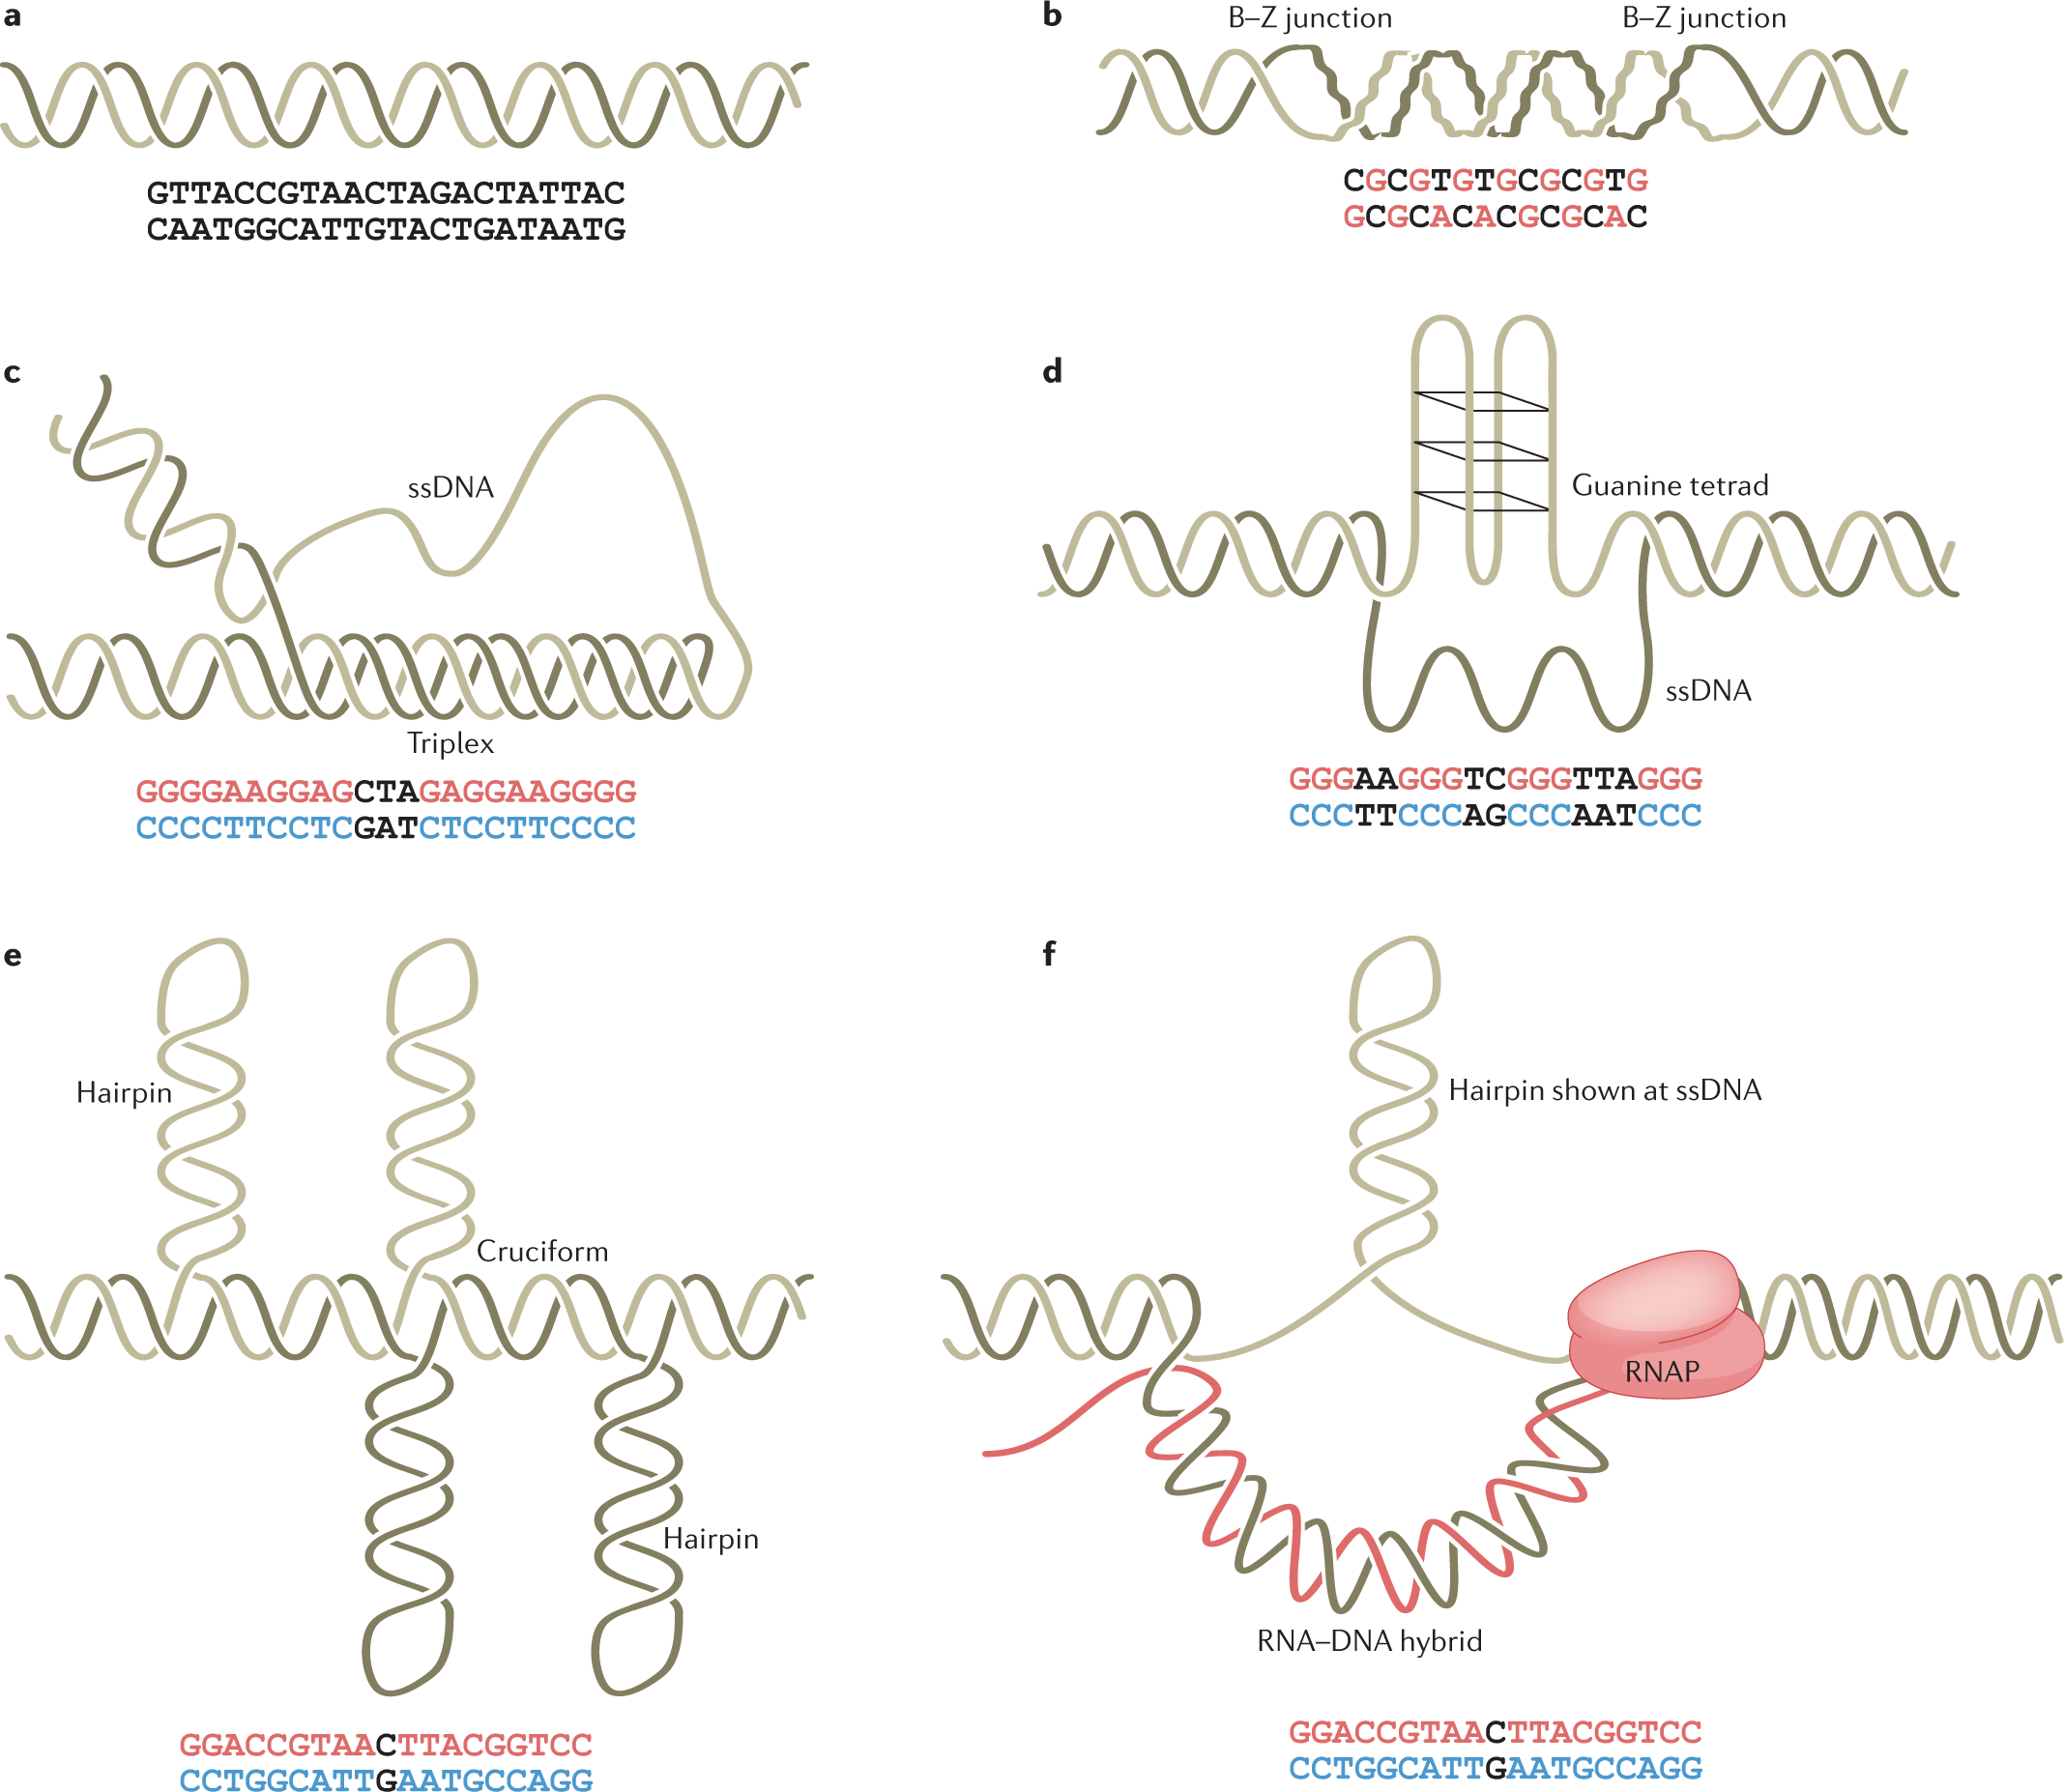
\includegraphics[width=9cm, height=6.5cm]{nonb_types.png}
	
	\footnotetext[3]{\tiny\cite{nijman2011synthetic,shen2018synthetic}}
	
	\end{frame}

	%Slide 6
	% Poly(ADP-ribose) polymerases (PARPs) repair DNA SSBs through the BER pathway. PARP inhibitors, such as olaparib, prevent repair by trapping the inactivated PARP onto the SSB, resulting in the generation of DNA DSBs during the replication process. In tumors with a homologous recombination deficiency (HRD), such as a BRCA1/2 mutation, the low-fidelity repair mechanism of NHEJ leads to increasing genetic instability and ultimately death of the tumor cell.
	\begin{frame}{Non-Canonical DNA Structures are Involved in Biological Processes}
		
		Non-B DNA structures have been shown to co-localize with \textcolor{blue}{functional genomic loci} (promoters, enhancers, etc) and \textcolor{blue}{genetic instability hotspots} \newline
		
		This suggests a role for non-B DNA in vital cellular events such as;
		\begin{itemize}
			\item Regulation of transcription
			\item Regulation of DNA replication and recombination
			\item Regulating genome integrity
		\end{itemize}
	
		\centering
		%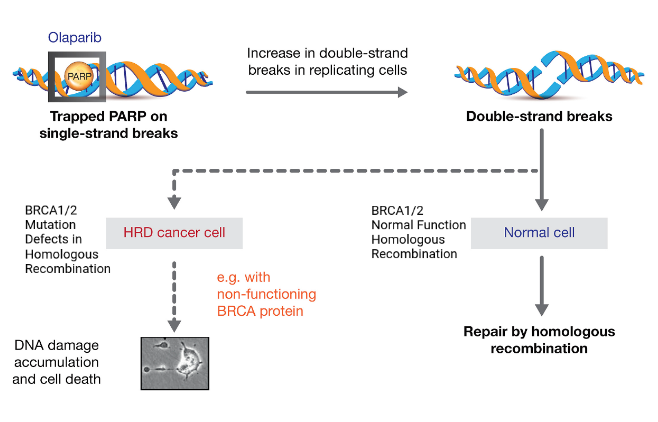
\includegraphics[width=8.5cm, height=6cm]{olaparib2.png}
		
		\footnotetext[4]{\tiny Figure From  \cite{o2015targeting}}
	\end{frame}

	%SLIDE 6 
	\begin{frame}{Diseases Associated with Non-Canonical DNA structures}
		
	\textbf{\color{blue}Repeat Expansion Diseases:} Expansions of non-B DNA structure-forming repeats have been implicated in many neurodegenerative and neuromuscular diseases. \newline
	
	\textbf{\color{blue}Genetic Instability Diseases:} Non-canonical DNA structures are associated with increased mutability (point mutations, deletions, insertions and chromosomal translocations)
	
	\begin{itemize}
		\item Enriched at chromosomal breakpoints in translocation-related cancers such as lymphomas and leukaemias.
		\item Can be recognized by DNA repair proteins, triggering error-generating repair processes
		\item G-quadruplexes are present within most human oncogenic promoters and at telomeres - a current theraputic target to downregulate transcription or block telomere elongation in cancer cells.
	\end{itemize}
	
	
	\end{frame}

	\begin{frame}{How are Non-B Structures Detected in the Genome?}
			\begin{center}
				\vspace{-1cm}
				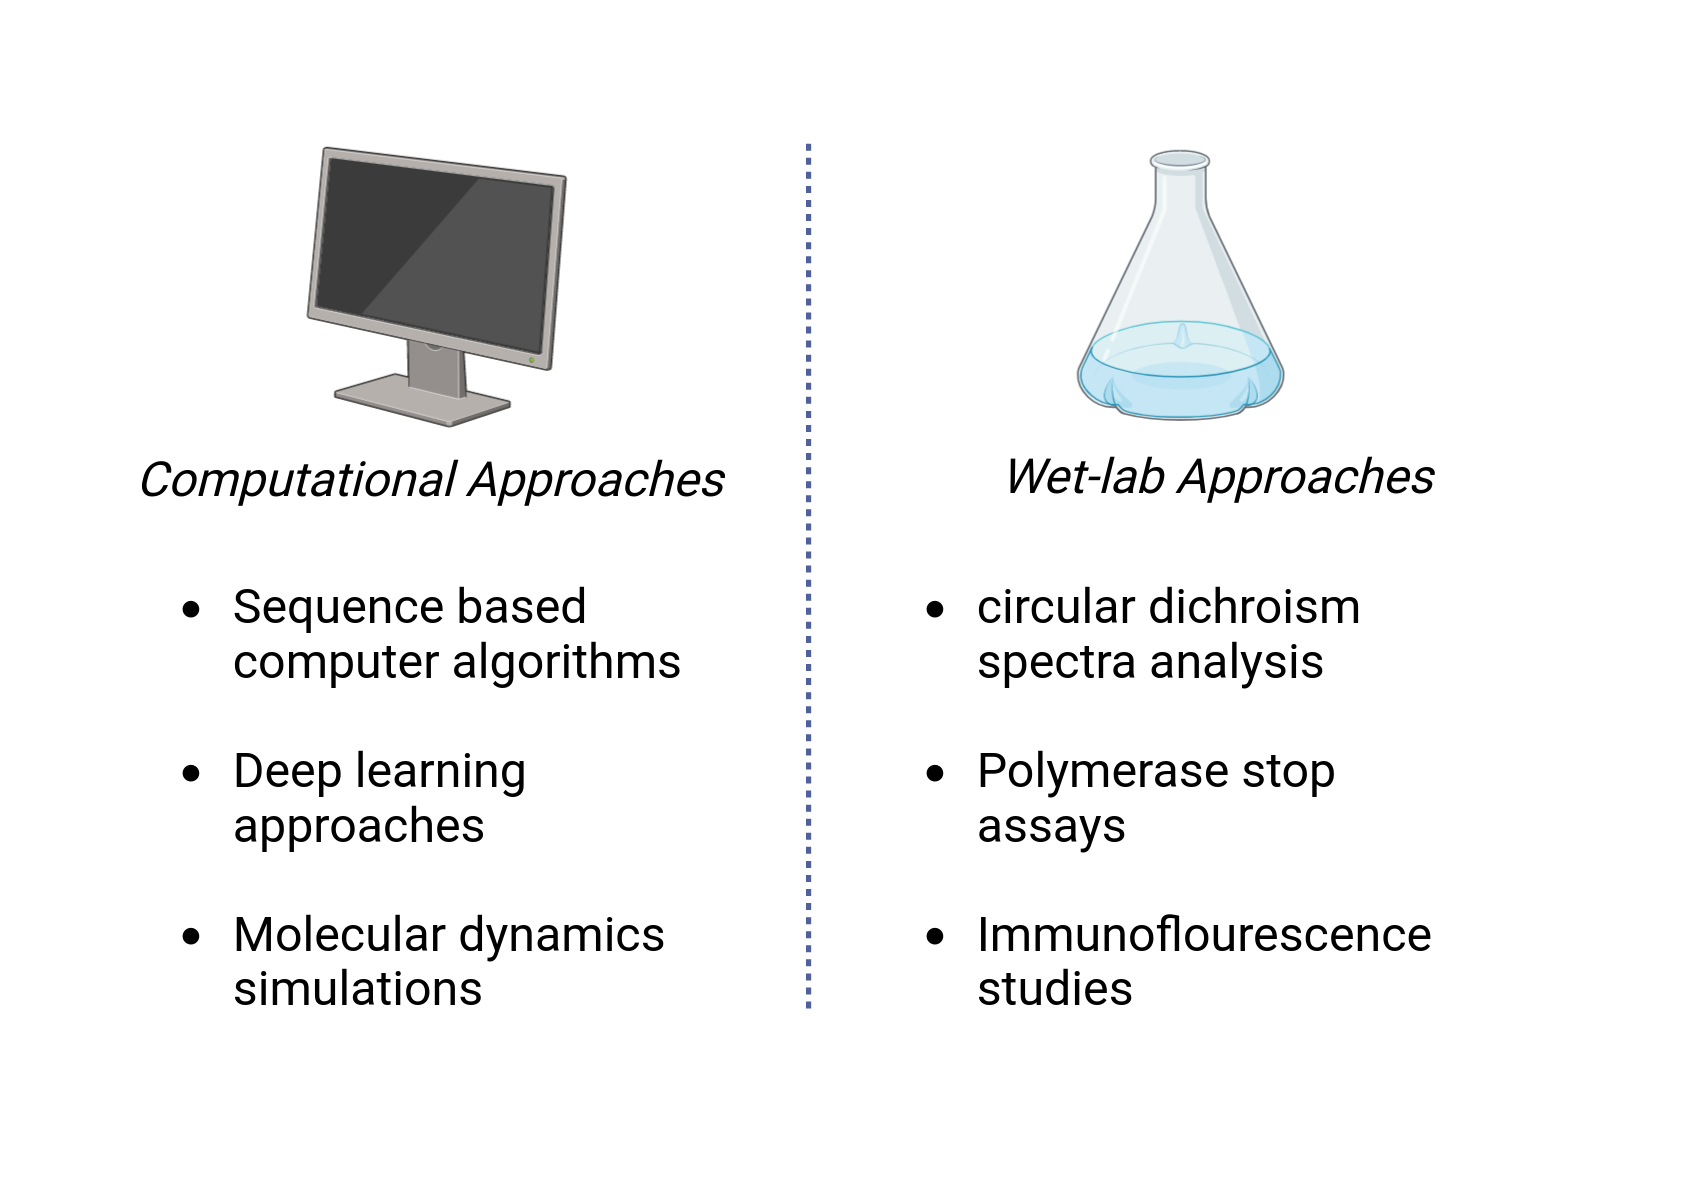
\includegraphics[width=12cm, height=8cm]{Predicting_nonb_structures.png}
				\vspace{-1.5cm}
			\end{center}
		These approaches are based primarily on \textcolor{blue}{DNA sequence motifs}, which are \textcolor{blue}{necessary}, but \textcolor{blue}{insufficient} for formation and are not available for all non-B DNA structures
		
		
	\end{frame}

	%%%%% APPRACH SECTION BEGINS HERE, 2 SLIDES

	\begin{frame}{Third Generation Sequencing: A Promising New Approach}
		\textbf{\color{blue}Single Molecule, Real Time Sequencing (SMRT):} Pacbio's third generation sequencing machine
		\begin{itemize}
			\item Emits a fluorescent pulse when nucleotide is detected - the time interval between two pulses is called the interpulse duration (IPD)
			\item Guiblet et al (2018), showed that there is a significant divergence between IPDs in non-B DNA motif regions compared to B-DNA regions
		\end{itemize}
		
		\centering
		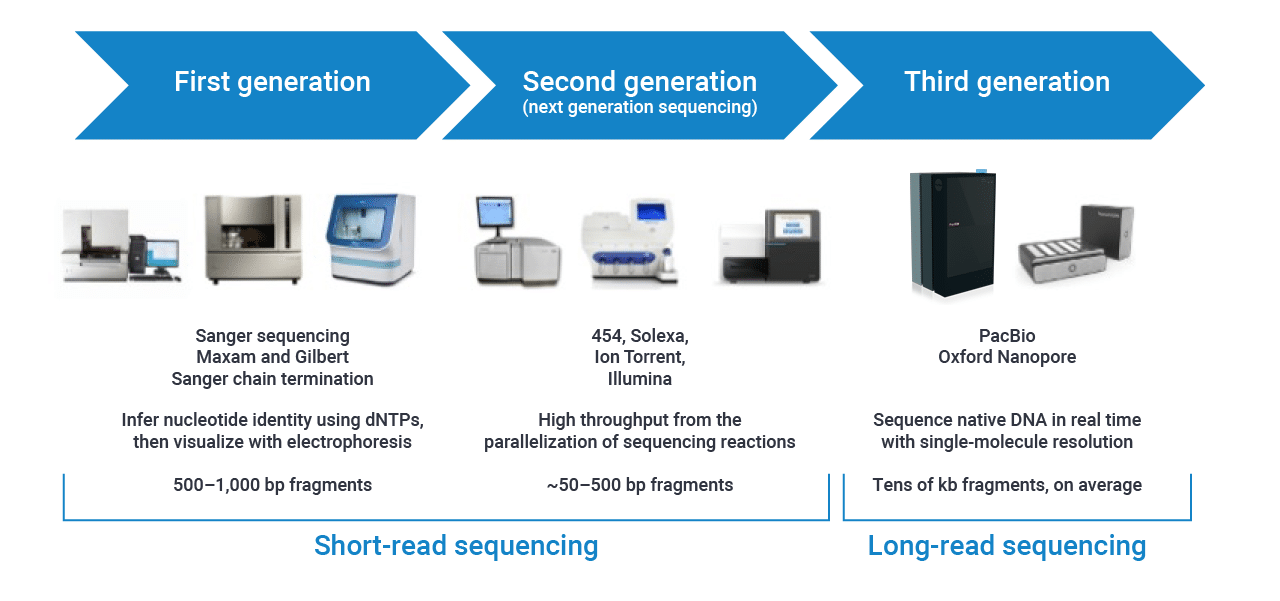
\includegraphics[width=10cm, height=4.5cm]{sequencing_evolution.png}
	\end{frame}

	\begin{frame}{Oxford Nanopore Sequencing Technology}
		\centering
		\begin{figure}[!htb]
			\centering
			\begin{minipage}{.3\textwidth}
				\centering
				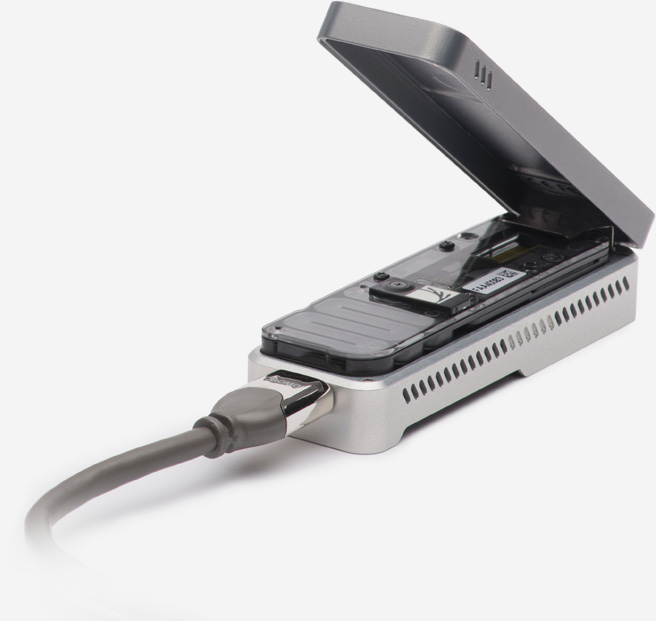
\includegraphics[width=3.5cm, height=6cm]{ont_machine.jpg}
				\caption{ONT Sequencer}
				\label{fig:prob1_6_2}
			\end{minipage}%
			\begin{minipage}{0.7\textwidth}
				\centering
				\movie[width=8cm, height=4.5cm]{placeholder box}{ont.mp4}
				\caption{Inside the Nanopore}
				\label{fig:prob1_6_1}
			\end{minipage}
		\end{figure}
		
			
	\footnotetext[5]{\tiny\cite{cheng2021synthetic}}
	\end{frame}

	\begin{frame}{Predicting Non-B Structures From Nanopore Sequencing}
		A recently published reference set of genome-wide cSLs common to many cancer types was utilized
		\begin{center}
				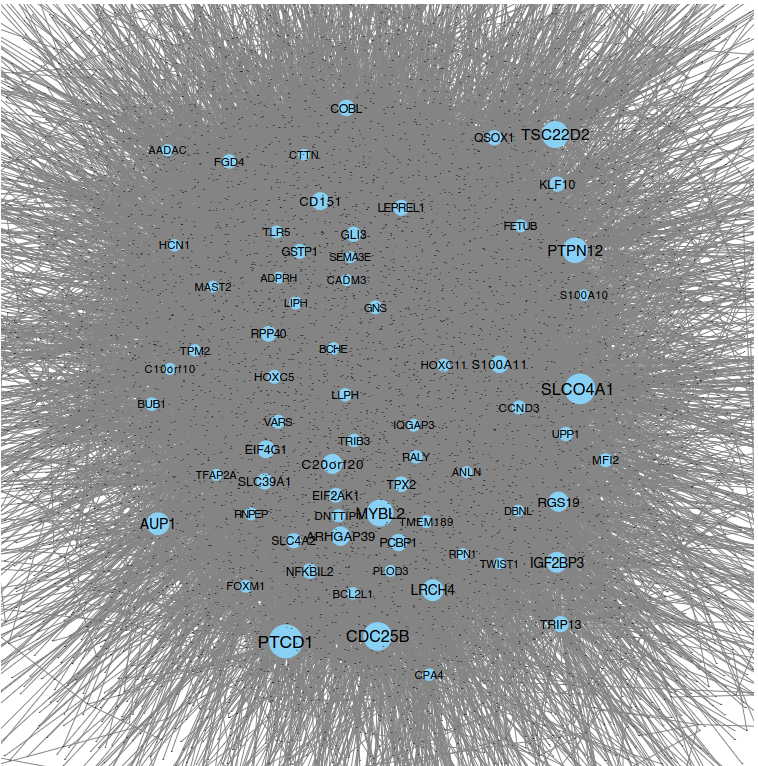
\includegraphics[width=6cm,height=6cm]{corenet.png}
		\end{center}
	\footnotetext[2]{\tiny\cite{lee2018harnessing}}
	\end{frame}

	%EXPLAIN THE PROCESS OF ISLE HERE
	\begin{frame}{Building Pan-Cancer Synthetic Lethality Networks}
		\centering
		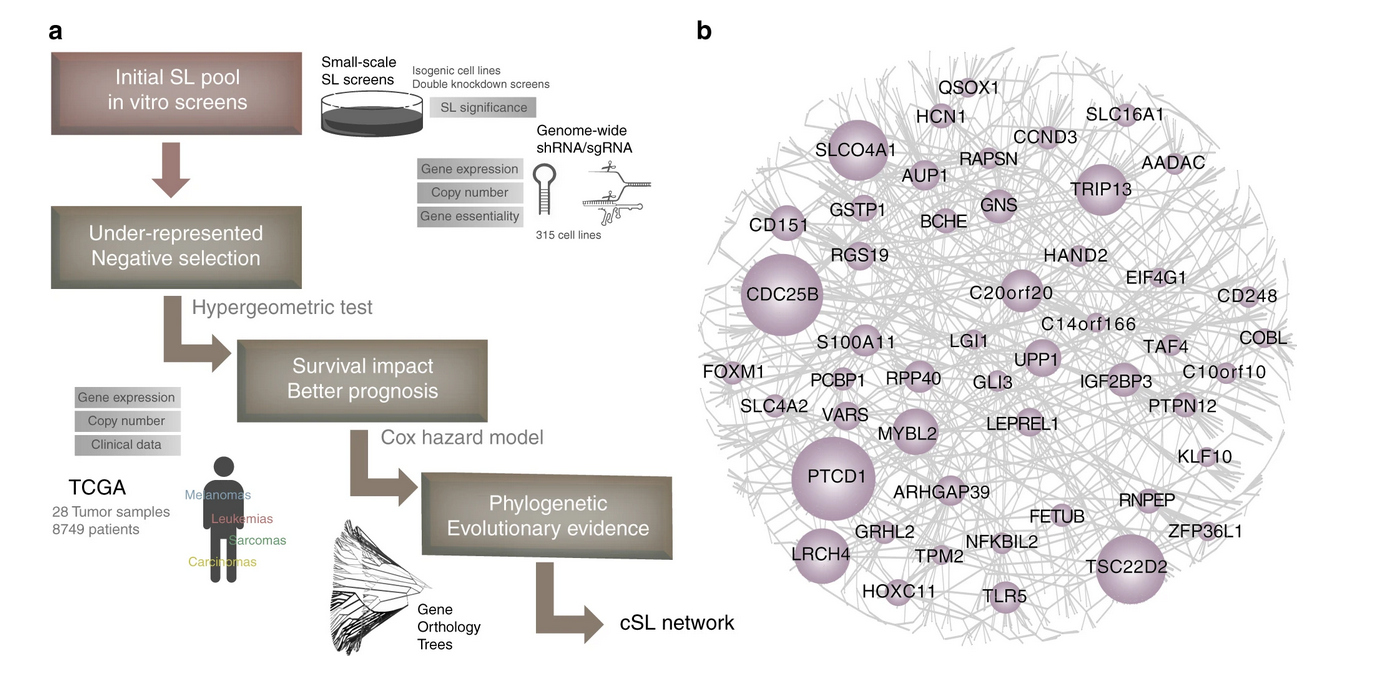
\includegraphics[width=13cm, height=7cm]{isle.png}
		%\movie[width=10cm,height=7cm,showcontrols=true]{\includegraphics[width=10cm, height=7cm]{pompe_thumbnail.png}}{pompe_trimmed.mp4}
		\footnotetext[2]{\tiny\cite{lee2018harnessing}}
	\end{frame}

	%%% EXPLAIN NSSE SURVEY A BIT
	%%% WHEN YOU TALK MENTION THAT THEY DID THIS SURVEY AFTER PLAYING THE GAME IN CLASS
	\begin{frame}{There is Variability in Synthetic Lethal Interactions Depending on Cancer Type}
		
		\textbf{\color{blue}Pan-Cancer Analysis:} Analysis of multiple types of cancer simultaneously, aims to identify commonalities shared across different types
		
		
		\textbf{\color{blue}Cancer-Specific Analysis:} Analysis of individual cancer types to better understand the variation within a specific cancer type \vspace{1cm}
		
		\begin{itemize}
			\item Pan-cancer analyses may overlook cancer-specific differences
			\item Availability of datasets for all cancer types varies, this may limit statistical power of pan-cancer analyses
		\end{itemize}
		
	\end{frame}

	%%%%RESULTS BEGIN HERE
	\section{Results}
	
	\begin{frame}{Sex Differences Add an Additional Layer of Complexity}
		Human sex differences are mainly caused by;
		\begin{enumerate}
			\item Gonadal hormone secretions
			\item Genes located on the sex chromosomes (X and Y) \newline
		\end{enumerate}
	This leads to differences in the frequency of certain cancer types and the efficacy of treatments in males and females
	\end{frame}

	\begin{frame}{Sex Differences Add an Additional Layer of Complexity}
		\centering
		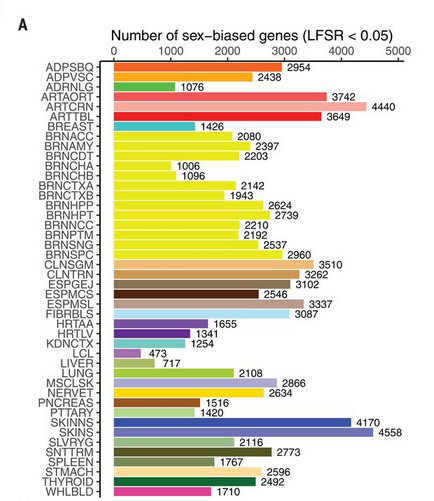
\includegraphics[width=6cm,height=7cm]{sex.png}
		\footnotetext[6]{\tiny\cite{oliva2020impact}}
	\end{frame}

	\begin{frame}{The Objective}
		\begin{center}
		%\includegraphics[width=11cm, height=6cm]{types_of_courses_taken.jpg}
		Can we build sex-specific synthetic lethality networks for various cancer types? \newline
		
		More specifically, we are trying to elucidate the differences in synthetic lethal interactions between males and females using a network based approach.
		\end{center}
	\end{frame}

\end{document}
